%-----------------------------------------------------------------------------
%
%    Domain Specific Identifiers
%
%-----------------------------------------------------------------------------


%\documentclass[preprint,authoryear]{acm_proc_article-sp}
%\documentclass{acm_proc_article-sp}
%\documentclass[preprint,authoryear]{acm_proc_article-sp}
%\documentclass[preprint,authoryear,10pt]{sigplanconf}

\documentclass[preprint]{sigplanconf}

\usepackage{ifthen}
\usepackage{pifont}
%\usepackage[small,compact]{titlesec}

% \usepackage{mathptmx}

% \usepackage{paralist}

% \usepackage[small,it]{caption}

\usepackage[pdftex]{graphicx}


%\usepackage{fancyhdr}


\usepackage{amsmath}
\usepackage{epigraph}
\usepackage[colorlinks=true,
        linkcolor=blue,
        citecolor=red,
        filecolor=black,
        urlcolor=black,
        bookmarks=true,
        bookmarksopen=true,
        bookmarksopenlevel=3,
        plainpages=false,
        pdfpagelabels=true]{hyperref}

%%--- listings configuration
\usepackage{listings}
\lstset{
  language={C},
  basicstyle=\ttfamily,
  keywordstyle=\bfseries,
  showstringspaces=false,
  commentstyle=,
  captionpos=below%,
%  numbers=left,
%  numberstyle=\tiny,
%  numbersep=5pt
}
\lstset{numberbychapter=false}

%\lstdefinestyle{L}{basicstyle=\ttfamily}
\lstdefinestyle{L}{basicstyle=\ttfamily\scriptsize}
\lstdefinestyle{numbers}
{numbers=left, stepnumber=1, numberstyle=\tiny, numbersep=10pt,basicstyle=\ttfamily\scriptsize}

%%--- end of listings configuration

%\pagestyle{fancy} 
% \sloppy

%\setlength{\parskip}{0pt}
%\setlength{\parsep}{0pt}
%\setlength{\headsep}{2pt}
%\setlength{\topskip}{0.1pt}
%\setlength{\topmargin}{1pt}
%\setlength{\topsep}{1pt}
%\setlength{\partopsep}{0pt}

\newboolean{showcomments}
\setboolean{showcomments}{true}



\ifthenelse{\boolean{showcomments}}
  {\newcommand{\mynote}[2]{
      {\color{red}
    \fbox{\bfseries\sffamily\scriptsize#1}
%       {\small$\blacktriangleright$\textsf{\emph{#2}}$\blacktriangleleft$}
       {\small \textsf{\emph{#2}} }
    % \marginpar{\fbox{\bfseries\sffamily#1}}
        }
   }
   \newcommand{\cvsversion}{\emph{\scriptsize $ $Revision: 1.42 $ $ -- $ $Date: 2005/10/01 00:23:32 $ $ }}
  }
  {\newcommand{\mynote}[2]{}
   \newcommand{\cvsversion}{}
  }

\newcommand{\here}{\mynote{***}{CONTINUE HERE}}
\newcommand\nb[1]{\mynote{NB}{#1}}
\newcommand\fix[1]{\mynote{FIX}{#1}}
% \newcommand\todo[1]{\mynote{TO DO}{#1}}
\newcommand\mpw[1]{\mynote{Marcel}{#1}}
\newcommand\rh[1]{\mynote{Robert}{#1}}

%\renewcommand{\topfraction}{0.85}
%\renewcommand{\textfraction}{0.1}
%\renewcommand{\floatpagefraction}{0.85}



\begin{document}
%\fontsize{9.7}{12}\rm

\linespread{0.9}

\conferenceinfo{SPLASH 2013}{date, City.} 
\copyrightyear{2013} 
\copyrightdata{[to be supplied]} 

%\titlebanner{banner above paper title}        % These are ignored unless
%\preprintfooter{short description of paper}   % 'preprint' option specified.


\title{Uniform Resource Access in Objective-Smalltalk with Polymorphic Identifiers}

%\author{Marcel Weiher\inst{1} \and Robert Hirschfeld\inst{2}}
%\institute{metaobject ltd. \email{marcel@metaobject.com} \and Hasso Plattner Institut \email{robert.hirschfeld@hpi.uni-potsdam.de}}


\authorinfo{Marcel Weiher}
           {metaobject ltd.}
           {marcel@metaobject.com}
\authorinfo{Robert Hirschfled}
           {Hasso Plattner Institut}
           {hirschfeld@acm.org}

%\numberofauthors{2}
%\author{
%\alignauthor Marcel Weiher\\
%       \affaddr{metaobject ltd.}\\
%       \email{marcel@metaobject.com}
%\alignauthor Robert Hirschfeld\\
%       \affaddr{Hasso Plattner Institut}\\
%       \email{}
%}

\maketitle

\begin{abstract}

In object-oriented programming, polymorphic dispatch of operations
decouples clients from specific providers of services and allows 
implementations to be modified or substituted without affecting clients. 

The Uniform Access Principle (UAP) tries to extend these qualities to 
resource access by demanding that access to state be indistinguishable
from access to operations.  Despite language features supporting the
UAP, the overall goal of substitutability has not been achieved for
either alternative resources such as keyed storage, files or web pages, or for alternate 
access mechanisms:    
specific kinds of resources are bound to specific access mechanisms and vice versa.
Changing storage or access patterns either requires changes to both clients and
service providers and trying to maintain the UAP imposes significant penalties in terms of
code-duplication and/or performance overhead.

We propose introducing first class identifiers as polymorphic names for storage locations
to solve these problems.  With these \emph{Polymorphic Identifiers}, we show that
we can provide uniform access to a wide variety of resource types as well as 
storage and access mechanism, whether parametrized or direct, without affecting
client code, without causing code duplication and improving performance significantly.

\end{abstract}

% \category{D.3.3}{Programming Languages}{Language Constructs and Features}

%\terms{language, design}
%\keywords{Polymorphic Identifiers} % NOT required for Proceedings
%\setlength{\epigraphrule}{0pt}

%-=-=-=-=-=-=-=-=-=-=-=-=-=-=-=-=-=-=-=-=-=-=-=-=-=-=-=-=-=-=-=-=-=-=-=%

\section{Introduction}

Imperative object oriented languages such as Smalltalk, C\#, Java or Objective-C provide
built-in storage for their objects in the form of instance variables.  These instance
variables 

Imperative programming languages such a Pascal or C clearly distinguish between
data access and procedure or function invocation at the language level.  Data 
access is via \emph{L-Values}, that is \emph{Locations} that point into a \emph{store}~\cite{StracheyFund}
and can be read or written, whereas procedures and functions can only be invoked.

\begin{itemize}
\item only one kind of state, others via procedural abstraction (I/O, hash-table, ...)
\item early OOP still has that distinction
\item conflicts with representation independence, so UAP
\item implementations of UAP:  remove state access / properties
\item Problem:  still not enough, state variants leak
\item 
\end{itemize}


Imperative programming languages feature the concept of a store with locations.
Locations or \emph{L-Values} are characterized by the essential features of having content 
(an associated R-Value) and 2 operations to access and update this value from the location,
the \emph{Load-Update-Pair} or \emph{LUP} (also Strachey).  Strachey decouples the definition of a store
from the notion of memory or addressability. 

The same goes for parametrized access via pointers, which are 
R-Values that represent locations.  Pointers are characterized by two polymorphic 
operations, \emph{Follow} and \emph{Pointer}.  

Programming languages such as Pascal or C implement the store as main memory, with
identifiers mediating access.  We can compose these identifiers, use them on the LHS and RHS
and partially use them for indirect access.  Computational abstraction is handled separately.

Object-oriented programming languages mostly maintain the distinction between computational
and storage abstraction, with polymorphism and most other abstraction mechanisms only
applying to computational abstraction.  The better support for abstraction afforded by 
the computational abstraction mechanism has led to storage abstraction being 
de-emphasized by convention (Java, C\#,..) or by removing it partially (Smalltalk) or 
entirely (Self, Newspeak) from the user-visible language, reducing the number
of concepts in the language.  



The Uniform Access Principle (UAP) was coined by Meyer to formalize this relationship:  
access to state should be indistinguishable from computation.  However, the current
implementations interpret this as applying only to state in instance variables of objects.






%-=-=-=-=-=-=-=-=-=-=-=-=-=-=-=-=-=-=-=-=-=-=-=-=-=-=-=-=-=-=-=-=-=-=-=%





\section{Non-uniform access}
\label{nonuniform}
%\epigraph{When programming a component, the right computation model for the component is the least expressive model that results in a natural program.}{Rule of Least Expressiveness.}

This section provides three resource access scenarios where uniform access is difficult to achieve
with standard mechanisms, leading to compromises and non-uniform access patterns in practical
code.  Please note that this section is not about exhaustively enumerating all possible solutions
or conclusively proving that no better solutions exist. Instead it highlights that for common and
simple situations, achieving the goals of the UAP is not necessarily simple and obvious, and
non-uniform solutions are often viable and commonly used alternatives.

\begin{table}
\center
\begin{tabular}{|l|c|c|} \hline
   & C\#  	 & Objective-C  		 \\\hline 
read property & {\tt c = a.b; }	 & {\tt c = a.b;  }		 \\\hline 
write property & {\tt a.b = c; }	 & {\tt a.b = c; }		 \\\hline 
send message & {\tt a.b(c);  }	 & { [a b:c]; }		 \\\hline 
\shortstack{{define property}\\{autogenerated}}  & \shortstack{ {\tt public int b} \\ { \{\tt get; set; \} }}  & \shortstack{{\tt @property int b;}\\{\tt @synthesize b;}}\\\hline 
\end{tabular}
\caption{C\# and Objective-C syntax}
\label{objc-syntax}
\end{table}

We use Objective-C in our examples because it has both properties and a ``message not understood''
hook for handling messages without implementing them.  Table~\ref{objc-syntax} shows basic
Objective-C syntax compared to C\#.  


\subsection{User-defined storage implementations}
\label{userdefined}
Although language features supporting the UAP make it easy to substitute a single 
instance variable with a pair of methods or vice versa, substituting custom stores,
and doing so wholesale, is more difficult.

For our examples, we will be using a trivial {\tt Person} class shown in Listing~\ref{personclassdef}
using Objective-C syntax with property definitions for attributes {\tt name} and {\tt age}.

\begin{figure}[htbp]
\begin{lstlisting}[style=numbers,label=personclassdef,caption=Person class.]
@interface Person : NSObject 
{}
@property NSString *name;
@property NSNumber *age;
...@end
@implementation Person
@synthesize name,age, ...;
@end
\end{lstlisting}
\end{figure}


Dictionaries provide a generic interface to access their contents, so they have
one method for retrieving objects by key and another method for storing objects
by key, in our example {\tt objectForKey:} and {\tt setObject:forKey:} whereas
object properties can be accessed using dot notation and the property name.
Listing~\ref{dict-vs-property1} summarizes the differences, it is clear that implementations
cannot simply be substituted as is.


\begin{figure}[htbp]
\begin{lstlisting}[style=numbers,label=dict-vs-property1,caption=Dictionary vs. Property.]
person.name;
person.name = newName;
person[@"name"];
person[@"name"] = newName;
\end{lstlisting}
\end{figure}

It should be noted that similar to C\# and Eiffel, the syntax in  Listing~\ref{dict-vs-property1}
is surface syntax only that is mapped by the compiler to the message sends shown in
Listing~\ref{dict-vs-messages}.  

\begin{figure}[htbp]
\begin{lstlisting}[style=numbers,label=dict-vs-messages,caption=Dictionary vs. Property.]
[person name];
[person setName:newName];
[person objectForKey:@"name"];
[person setObject:newName forKey:@"name"];
\end{lstlisting}
\end{figure}

There are three basic options for bridging the gap and making access uniform between the
dictionary and the object:
\begin{enumerate}
\item  Listing~\ref{compatibility1} adapts the object to the dictionary's protocol by
	 implementing {\tt objectForKey:} and {\tt setObjectForKey:} and mapping the keys
	 to properties.
\item Listing~\ref{compatibility2} adapts the dictionary to the object's protocol by 
	implementing cover methods for every potential attribute that is to be stored.
\item Listing~\ref{compatibility3} also adapts the dictionary to the object's protocol, but
	this time by implementing the "forwardInvocation:" error handler that is invoked
	when a message is not understood by an object.
\end{enumerate}

None of these options is particularly appealing, as they all involve either performance penalties,
repetitive code or both.
	
\begin{figure}[htbp]
\begin{lstlisting}[style=numbers,label=compatibility1,caption=Making an object dictionary-compatible.]
-objectForKey:aKey
{
  if ( [aKey isEqual:@"name] ) {
    return self.name;		
  } else if ( [aKey isEqual:@"age] ) {
    return self.age;
  } else if ...
  }
}
-setObject:newObject forKey:aKey 
  if ( [aKey isEqual:@"name] ) {
    return self.name=newObject;		
  } else if ( [aKey isEqual:@"age] ) {
    return self.age=newObject;
  } else if ...
  }
}
\end{lstlisting}
\end{figure}

Adopting the dictionary's protocol as in Listing~\ref{compatibility1} as the uniform interface between
clients and their service providers means 
that the language's built in notations for access will no longer be used for interfacing between
objects, rather {\tt objectForKey:} and {\tt setObject:forKey:} will now be used universally.  In addition
to bloating client code and making it virtually unreadable, this also means having to implement
the {\tt objectForKey:}/{\tt setObject:forKey:} methods for every object.  These methods are not just
boilerplate that duplicates the already-existing property definitions, they are also more than an order
of magnitude slower than the built-in access, and slower even than dictionary access.  This 
performance overhead is imposed by the API, it cannot easily be removed by clever implementations.

In combination, these aspects of this solution strongly discourage object-modeling, as just using 
dictionaries everywhere is not just less code, but also faster than introducing objects.

\begin{figure}[htbp]
\begin{lstlisting}[style=numbers,label=compatibility2,caption=Making a dictionary object-compatible.]
-(NSString*)name
{
    return [self objectForKey:@"name];
}
-(void)setName:(NSString*)newName
{
  [self setObject:newName forKey:@"name];
}
-(NSNumber*)age
{
    return [self objectForKey:@"age"];
}
-(void)setAge:(NSNumber*)newAge 
{
  [self setObject:newName forKey:@"age"];
}
...
\end{lstlisting}
\end{figure}

The second option is to keep property access as the universal interface, mapping to dictionaries
inside the object using cover methods as shown in Listing~\ref{compatibility2}.  The advantages
of this approach are that we do no abandon the language-defined interface facilities and
there is no performance overhead imposed by the API.  The disadvantage is obvious from
Listing~\ref{compatibility2}:  introduction of duplicated boilerplate code on a massive scale.

Although independent identifiable concerns are supposed to be isolated in a single module~\cite{Parnas72},
and object-orientation is supposed to help us with this goal,
this ``storage concern'' is now spread all over the code-base.  If we want to change storage
from instance variables to dictionaries or back for a variety of objects, we must modify all
the objects involved, introducing or removing these cover methods as needed. 


\begin{figure}[htbp]
\begin{lstlisting}[style=numbers,label=compatibility3,caption=Compatibility via forwardInvocation.]
-(void)forwardInvocation:(NSInvocation*)inv 
{
  SEL sel=[inv selector];
  NSString *msg=NSStringFromSelector( sel );
  if ( [msg hasPrefix:@"set"] ) {
    NSRange  r      = NSMakeRange(3,1);
    NSString *first = [msg substringWithRange:r];
    NSString *rest  = [msg substringFromIndex:4];
    NSString *key   = nil;
    id arg=nil;
    [inv getArgument:&arg atIndex:2];
    first=[first lowercaseString];
    key=[first stringByAppendingString:rest];
    [self setObject:arg forKey:key];
  } else {
    id result=[self objectForKey:msg];
    [inv setResult:&result];
  }
}
...
\end{lstlisting}
\end{figure}

In dynamic languages, we have a third option, using the error handler invoked when a method
is not found to simulate the cover methods without having to implement them, as shown
in Listing~\ref{compatibility3}.   Although this approach does reduce the need to write
cover methods for each individual attribute, it still needs to be implemented for every keyed
access class or injected if injection facilities are available.  The fact that it must convert
distinct message message names to keys via string processing not only makes it fragile,
but also quite slow, at around three orders of magnitude slower than a plain message
send accessing an attribute.

Although we have shown three possible ways of honoring the UAP when dealing with custom
attribute storage in Objective-C, all of them come with
serious drawbacks, and so the fourth, not previously listed option is usually chosen:  simply
live with non-uniform access for custom stores.

Other object-oriented languages such as C\#, Scala, Python, Ruby, Eiffel, Java and Smalltalk,
present the developer with the same tradeoffs, though details vary slightly and the dynamic
message resolution technique from Listing~\ref{compatibility3} is only available in the dynamic
languages. 

The problems presented apply to any custom store, not just dictionaries,
because any custom store has to identify the storage locations (\emph{L-Values}) to reference,
so it has to translate from messages to \emph{L-Values} and back somehow.  Furthermore,
they are transitive:  they apply just as much if we hide a custom store inside of an object as
they do when we substitute the custom store directly for the object.

  Special 
machinery is sometimes available to perform this translation for instance variables (in the form of 
properties in C\#, Python and Objective-C, in the form of aliases in Eiffel and Scala and hidden
in Self), but these mechanism only apply to instance variables, not to custom stores.



\subsection{Parametrized access}
\label{parametrized}
Another source of non-uniformity is the difference between direct access, where the attribute
to be accessed is known at compile time and present in the source code, and parametrized
access, where the exact attribute is passed as a parameter at run time.  Parametrized access
is frequently used in UI toolkits, serialization and persistence mechanisms in order to generically
access attributes of an object.  For example, a
UI text field is parametrized in order to be able to read and write the {\tt name} attribute of
an object.

Table~\ref{direct-vs-parametrized}
summarizes how read and write access to an attribute differs between direct and parametrized
access in Objective-C.  Property access is the simplest, as there simply is no parametrized variant
available.  Keyed access can use the same message format for indirect and direct access, and
more crucially, the same key for both read and write access.  Message-based access, on the
other hand, must not only switch from the direct messaging syntax to indirect {\tt perform:}
messages, but also must provide two different message selectors, the read and the write
selector (e.g. {\tt name} and {\tt setName:}).

\begin{table*}[htbp]
\center
\begin{tabular}{|r|c|c|} \hline
   &  direct	 & parametrized  		 \\\hline 
property read 	 &   {\tt person.name;  }	&  -	 \\\hline 
property write 	 & {\tt person.name=newName; }	 & -		 \\\hline 
message read 	 &  {\tt  [person name]; }	 & {\tt [person perform:readAttrSel]; }		 \\\hline 
message write 	 & {\tt  [person setName:newName]; }	 & {\tt [person perform:writeAttrSel with:newName]; }		 \\\hline 
keyed read  & {\tt person[@"name"]; }	 & {\tt person[anAttribute];  }  \\\hline 
keyed write  & {\tt person[@"name"]=newName;}	 & {\tt person[anAttribute]=newName; }		 \\\hline 
\end{tabular}
\caption{Direct vs. parametrized access}
\label{direct-vs-parametrized}
\end{table*}


In order to have parametrized read/write access to an attribute, we again seem to have effectively
three options:

\begin{enumerate}
\item Use dictionaries or another keyed store exclusively when parametrized access is required
\item Map a keyed API to message-sends dynamically (Option 2 of Section~\ref{userdefined}).
\item Implement an ``L-Value Reference'' object that either captures or dynamically derives 
	the two message required to access the specified attribute relative to an object.
\end{enumerate}


Option 1 leads to either non-uniform access or standardizing on dictionaries and foregoing 
object-oriented modeling.   It also means that even direct access, with all values known
at compile-time, must use the same run time access path, with the order-of-magnitude
performance penalty.
 
Option 2 is an option, but due to the negative performance
consequences we looked at in
Section~\ref{userdefined} not a good one.   Option 3,  performing the computation of the selectors
in an object and reusing that object has the potential of being much faster. 

\begin{figure}[htbp]
\begin{lstlisting}[style=numbers,label=valueacessor,caption=Class encapsulating message-based attribute access.]
@interface ValueAccessor : MPWObject
{
  id target;
  NSString *attributeName;
  SEL         getSelector,putSelector;
}
@property (strong) NSString *attributeName;
-initWithTarget:aTarget attribute:(NSString*)attrName;
-value;
-(void)setValue:
@end
@implementation ValueAccessor
@synthesize attributeName;
-initWithTarget:aTarget attribute:(NSString*)attrName
{
  self=[super init];
  getSelector=NSSelectorFromString( attrName );
  NSString *setName=[attrName capitalizedString];
  setName=[setName stringByAppendingString:@":"];
  setName=[@"set" stringByAppendingString:setName];
  putSelector=NSSelectorFromString( setName );
  return self;
}
-value
{
  return [self perform:getSelector];
}
-(void)setValue:newValue
{
  [self perform:setSelector with:newValue];
}
\end{lstlisting}
\end{figure}

A {\tt ValueAccessor} class implementing this idea is shown in Listing~\ref{valueacessor}.  However, 
as demonstrated in Listing~\ref{valueacessoruse}, using this
{\tt ValueAccessor} class is significantly more verbose and less convenient than just using the 
direct keyed access method of option 2.  This means that it is unlikely to be used in a direct-use
setting, so transformation from direct to parametrized use implies a large change in client code.

In addition, we have to take into account the findings from
Section~\ref{userdefined}, which concluded that we are likely to not have uniform access based on
messages only, which option 3 relies on.  

\begin{figure}[htbp]
\begin{lstlisting}[style=numbers,label=valueacessoruse,caption=Keyed access vs. using a ValueAccessor]
a = [person objectForKey:@"name];
id valueAccessor = [[ValueAccessor alloc]
           initWithTarget:person 
           attributeName:@"name"];
a = [valueAccessor value];
\end{lstlisting}
\end{figure}

Again, we find that although we have several solutions that offer different trade-offs, no obvious
method presents itself for achieving uniformity of access when parametrized access is involved.
In fact the problems of not having uniform direct access compound the problems of parametrized access.


\subsection{External resources}

Interaction with resources outside the application's memory space keeps increasing
in importance,
for example Apple's Pages DTP application has 3.9MB of compiled code,
but 250MB of non-code resources in 18792 files (not counting frameworks), and
mobile applications are often just thin wrappers around web-resources accessible
via HTTP~\cite{http}.  However, API and language support
for abstracting over such resources is limited.  In a way that is similar to the custom stores we looked at in Section~\ref{userdefined}, languages make it difficult to create APIs that separate concerns
and respect the UAP.

Listing~\ref{imagefromfile} shows loading an image file from a file using a convenience
API.   An instance of the {\tt NSBitmapImageRep} class is initialized by reading the file
from the absolute file-system path {\tt /Users/john/button.png}.

\begin{figure}[htbp]
\begin{lstlisting}[style=numbers,label=imagefromfile,caption=Accessing an image from the file system]
image = [[NSBitmapImageRep alloc] 
        initWithContentsOfFile:@"/Users/jo/button.png"];
\end{lstlisting}
\end{figure}

Rather than hiding implementation details and allowing
 them to be varied independently, the API used in Listing~\ref{imagefromfile} requires the caller
to expose and determine virtually all implementation details right at the call site:

\begin{enumerate} 
\item The fact that we are loading data from a filesystem
\item The name of the image and the full access path to the image, encoded as a literal string, so
	the API assumes that strings are filesystem paths
\item The fact that the image is encoded in the PNG file format
\item The class that will be used to represent the image in code
\end{enumerate}

If we wish to separate the resource name from its access path, we need to do string 
processing to combine the two back into a full path.  Using relative paths is dangerous
at best because those are relative to the current working directory, which is global to
the process and not necessarily predictable.

If we wish to load the image from the web rather than from the local filesystem, we need to
change APIs, as shown in Listing~\ref{imagefromweb}.  Being URI-based, the
API in this example can also be used to load images from the filesystem, but its additional
complexity and verboseness make the previous convenience API preferable as long as
it is sufficient.

\begin{figure}[htbp]
\begin{lstlisting}[style=numbers,label=imagefromweb,caption=Loading image from web]
uristring = @"http://example.com/button.png"
imaguri = [NSURL URLWithString:uristring];
data = [NSData dataWithContentsOfURI:imageuri];
image = [[NSBitmapImageRep alloc] initWithData:data];
\end{lstlisting}
\end{figure}

Similarly, if we decide to use a vector file format such as PDF, we need to change the
class to {\tt NSPDFImageRep} and the file name.  Finally, if we decide to create the
image programmatically rather than loading it from a file, we must change to 
a message send {\tt [imageProvider button];}.

We can improve the situation a little by introducing a {\tt Resourcer} class like the
one shown in Listing~\ref{resourcer}, which hides differences between different
access methods and base paths, exposing just the resource name itself. 

\begin{figure}[htbp]
\begin{lstlisting}[style=numbers,label=resourcer,caption=Resourcer implementation]
@interface Resourcer : NSObject
{
        NSURL *baseURL;
}
-initWithBaseURLString:(NSString*)str;
-objectForKeyedSubscript:key;
-(void)setObject:newValue forKeyedSubscript:key;
@end

@implementation Resourcer

-initWithBaseURLString:(NSString*)str
{
    self=[super init];
    baseURL=[NSURL URLWithString:str];
    return self;
}
-(NSURL*)urlForRelativePath:(NSString*)path
{
    return [NSURL URLWithString:path relativeToURL:baseURL];
}
-objectForKeyedSubscript:key
{
    NSURL *loc=[self urlForRelativePath:key];
    return [NSData dataWithContentsOfURL:loc];
}
-(void)setObject:newValue forKeyedSubscript:key
{
    NSURL *loc=[self urlForRelativePath:key];
    [newValue writeToURL:loc atomically:YES];
}
@end
\end{lstlisting}
\end{figure}

Once we have an initialized {\tt Resourcer} instance, access to a specific resource
is  simple:   {\tt button = resources[@"button.png"];}   With an additional {\tt Mapper}
(not shown) we can map specific resource types to classes, so retrieving a 
resource using the syntax above doesn't just return raw bytes but initialized 
instances.  

However, as {\tt resource[@"button.png"]} is still syntactically different from {\tt [resource button]},
our solution does not conform the UAP, so if we decide to compute the button image instead
of using a pre-rendered version, we still need to change client code.   We have the same three options  discussed
in Section~\ref{userdefined} for bridging
the gap:  (1) standardize on dictionary syntax, (2) create individual cover methods or
(3) use a message error handler.  

In addition to the problems with these solutions already discussed,
using messaging to access external resources by name has the additional issue that 
resource names frequently don't conform to language messaging syntax, so either
some resources are unreachable or some mapping must be created and maintained.

Furthermore, paths with multiple components are difficult to map to messaging without
running into stratification issues:  either the messages are immediately resolved to
a resource, in which case paths with multiple components cannot be expressed, or
the messages just build a path, which must then be resolved to an actual resource
separately, preferably using a message name that doesn't conflict with a potential
path component. 



\subsection{Problem Statement Summary}

Although we  managed to conform fully or at least partially to the UAP in most
of these examples in the end, the results have been highly unsatisfactory.  Why?   
First, the significant issues identified with these solutions make it unclear if
conforming to the UAP is worth the cost.  Secondly, the very diversity of the
solutions, with little to clearly mark one as favorite, works against the 
uniformity that the UAP is trying to achieve.

As we saw in Sections~\ref{userdefined} and \ref{parametrized}, the difficulty
we had with custom stores and references was having to map between 
a message that performs an operation on a specific L-Value ({\tt setName:})
and the combination of the  L-Value itself ({\tt name}) and the operation ({\tt set:}).

Language support for the UAP automates this mapping, but only in a few
special cases:  when the store being mapped to is instance variable storage
and when the external access is direct.  In all other cases, some of which
we have examined, existing language support is insufficient and the
UAP unravels.


%-=-=-=-=-=-=-=-=-=-=-=-=-=-=-=-=-=-=-=-=-=-=-=-=-=-=-=-=-=-=-=-=-=-=-=%

\section{Polymorphic Identifiers}
\label{polymorphic-identifiers}

\emph{Polymorphic Identifiers} extend the equivalence between storage and 
computation promised by the UAP from built-in instance variable storage
to user-defined stores including the filesystem and remote storages such
as the web.




Polymorphic Identifiers generalize direct references by combining the techniques for resource access
discussed in the previous section such as reifying the identifier lookup process and using messaging 
to make it polymorphic, in addition to expanding identifier syntax to accommodate extension and 
opening up the language for extension at this point  with open-implementation techniques~\cite{OpenImplementations}.




The syntax for accessing these different types of resources is identical, even if the actual
names differ, and storing values into the resources is always accomplished using the assignment operator.
As it is possible to (re-)bind scheme names to existing or new schemes, all these different access 
mechanism are interoperable and can be substituted for one another.

The Polymorphic Identifier approach consists of three basic parts:
\begin{enumerate}
\item \emph{Polymorphic Identifiers} themselves are URIs\footnote{Other syntax variants such as dot notation should also work.}.
	  They are typically created by the 
	compiler and have a structured runtime representation that can be manipulated
	at a semantic level rather than as character strings, so consistency can be 
	maintained.
\item \emph{Scheme-handlers} manage a set of resources and, when registered,
	 the namespace that is associated
	with them.  They primarily turn \emph{Polymorphic Identifiers} into \emph{references} and
	are created by developers, with a basic set provided by the environment.
\item \emph{References} are created and used transparently by the run-time and compiler
	to mediate access to the specific resource identified by a \emph{Polymorphic Identifier}.
	
	
\end{enumerate}

All three elements are plain objects that only become part of the language when registered
with the compiler or runtime.

Figure~\ref{scheme-eval} shows the generic identifier lookup of Figure~\ref{identifier-eval}
extended to Polymorphic Identifiers.  The basic mechanism is still the same except for the
addition of \emph{scheme-handlers} mediating the lookup process.  The left hand side of the
diagram corresponds to the lookup in Figure~\ref{identifier-eval}, with the difference that
the lookup that was previously hardwired into the language is now mediated by the {\tt var}
scheme-handler, which in turn was selected by the {\tt var} scheme that's part of the 
Polymorphic Identifier.


\begin{figure}[htbp]
\centering\includegraphics[scale=0.45,page=1]{scheme-evaluation.pdf}
\caption{Polymorphic Identifier lookup from two schemes}
\label{scheme-eval}
\end{figure}


The right hand side of Figure~\ref{scheme-eval} shows fetching of a web-resource from
a remote server following the same four step lookup process, with the following steps:

\begin{enumerate}
\item a character sequence is turned into a Polymorphic Identifier,
\item the scheme part of the polymorphic handler is used to select a scheme-handler, in this case the {\tt http} handler,
\item the scheme-handler evaluates the \emph{scheme-specific} part of the Polymorphic Identifier ({\tt //deepThought.org/theAnswer})
	 and returns a reference, in this case a web-reference,
\item this (web-)reference mediates access to the actual resource, in this case translating requests to store or retrieve the 
	resource into HTTP GET or PUT requests via an http client library.
\end{enumerate}

These four steps can happen at compile-time or run-time and can be partially completed.
A reference to a local stack variable, for example, will typically have none of the
three components visible at run time, with all that remains being optimized 
machine code to directly access the resource (the stack variable).
A file or web-reference, on the other hand, will typically have the Polymorphic Identifier itself
compiled, with evaluation deferred until runtime.  Finally, there are facilities
for turning strings into Polymorphic Identifiers at runtime.


\section{Schemes and scheme-handlers}
\label{schemes}
The addition of \emph{schemes} to identifiers in order to distinguish different kinds of resources
and resource access represents
the major addition that \emph{Polymorphic Identifiers} bring to a programming language.
Each scheme is backed by a \emph{scheme-handler}.  Scheme-handlers broadly fall into two categories:
 \emph{primitive schemes} (Section~\ref{primitiveSchemes})
directly encapsulate access to some sort of resource, while \emph{composite schemes} (Section~\ref{compositeSchemes})
can be used to build new schemes out of existing schemes, forming a scheme algebra.

\sloppy   % FIXME

Scheme-handlers are represented by normal objects that respond to a well-defined protocol 
accessible by user level code.  They
become part of the language by binding them to a particular scheme, after which
all \emph{Polymorphic Identifiers} with that scheme will be resolved using that particular scheme-handler.
The {\tt scheme:} scheme manages the mapping of scheme-names to scheme-handlers, so the code 
{\tt scheme:http := URLSchemeResolver scheme} binds an instance of the {\tt URLSchemeResolver} class
to the {\tt http:} scheme.

\fussy

 Any scheme-handler
can be used for any scheme-name, as long as it implements the handler protocol
compatibly.


The \emph{scheme scheme} can also be queried,
so the expression {\bf scheme:http} returns the currently installed http handler, and 
{\bf scheme:scheme} returns the scheme scheme itself, which will list the currently
installed schemes.  Listing~\ref{scheme-scheme} shows the schemes installed by
default in the scripting environment {\tt stsh}.

\vspace{-0.5em}
\begin{figure}[htbp]
\begin{lstlisting}[style=numbers,label=scheme-scheme,caption=List of schemes via scheme:scheme.]
> scheme:scheme 
scheme-resolver with the following schemes: (defaults,  env, class,
    file, ftp,  http, https   default, var, sel,    scheme,    bundle,  mainbundle   )
\end{lstlisting}
\end{figure}
\vspace{-0.5em}

To illustrate the concepts, we will now present a few built-in scheme-handlers, ways to construct new
scheme-handlers out of existing scheme-handlers and apply these scheme-handlers to common
problems.

\subsection{Primitive Schemes}
\label{primitiveSchemes}

Primitive schemes are endpoints, they directly
mediate access to a specific kind of resource, often using a separate
library such as {\tt libwww} or {\tt libcurl}.  Primitive schemes
subsume both what is normally considered variable access and 
what is usually considered I/O, network and filesystem access.


\subsubsection{External resources}
\label{externalResources}

The list of default scheme-handlers in Listing~\ref{scheme-scheme} contains a few familiar URI schemes:
{\tt http}, {\tt https}, {\tt ftp}, and {\tt file}.   These behave in the expected way:   referencing them in an expression will
retrieve the bytes from the web-server, FTP-server or file, and placing them on the left hand side of
an assignment statement will perform an HTTP or FTP PUT request or write to a file system. 
 
Listing~\ref{download-to-file} shows how an RFC can be downloaded directly from a web-site
to a file, or how the web page could be updated given the right permissions, and demonstrates how integrating both filesystem access and the web as first class datatypes
goes some way to closing the gap between application programming languages and so called
scripting languages.

\begin{figure}[htbp]
\begin{lstlisting}[style=numbers,label=download-to-file,caption=Downloading an RFC to a file.]
file:rfc1738:=http://datatracker.ietf.org/doc/rfc1738.
http://datatracker.ietf.org/doc/rfc1738:='New RFC'.
\end{lstlisting}
\end{figure}

In fact,  Objective-Smalltalk is used as a Unix scripting language using the {\tt stsh} command
interpreter for interactive and batch use with only minor adaptations to this use-case such
as semi-automatic parameter and return-value adaptation.


The {\tt stcat} script in Listing~\ref{stcat} prints an arbitrary resource to Unix standard output, 
similar to the way the Unix {\tt cat} command is used to display files\footnote{{\tt stcat} only 
displays a single resource rather than concatenating several.}.
The declaration of the {\tt stcat} script as a method in line 2 enables the infrastructure to 
handle some interfacing tasks such as argument and return value conversion, as well
as making it possible for the script to be loaded and used as an actual 

The {\tt ref} type of the {\tt file} parameter means that this parameter will be bound to the
reference that results from evaluating the Polymorphic Identifier passed as a command
line parameter.    Line 3 simply retrieves the value of the reference and returns it as
the return value of the method, which the scripting environment knows to print to {\tt stdout}.


\begin{figure}[htbp]
\begin{lstlisting}[style=numbers,label=stcat,caption={\tt stcat} prints contents of any resource.]
#!/usr/local/bin/stsh
#-stcat:<ref>file
file value.
\end{lstlisting}
\end{figure}


The command  {\tt stcat http://datatracker.ietf.org/doc/rfc1738} shows \break \mbox{Request}
For Comment 1738 (RFC) from the web site of the rfc-editor, whereas 
the command {\tt stcat file:\~\//.bashrc} will display the user's bash startup script, assuming you are a user of the
bash shell, and on a Unix system, {\tt stcat env:HOME} will print the path to 
your home directory.
\fussy

With a current Unix shell each of these resource types would have used a different
access syntax or command:   {\tt curl http://datatracker.ietf.org/doc/rfc1738} for the
web resource, {\tt cat  \~\//.bashrc} for the file and {\tt echo \$HOME} for the environment
variable, as would using Objective-Smalltalk without Polymorphic Identifiers .

The {\tt scurl} command in Listing~\ref{scurl} is slightly more complicated than {\tt stcat} because
it needs to manipulate the identifier.  The {\tt scurl} command
is the {\tt stsh} variant of the {\tt curl -O} command for downloading files from the web, giving 
{\tt scurl} the argument {\tt http://http://datatracker.ietf.org/doc/rfc1738} will download the specified web resource
to the current directory as the file {\tt rfc1738}.


\begin{figure}[htbp]
\begin{lstlisting}[style=numbers,label=scurl,caption={\tt scurl} downloads files.]
#!/usr/local/bin/stsh
#-<void>scurl:<ref>urlref
fileName:= urlref identifier lastPathComponent.
file:{fileName} := urlref value.
\end{lstlisting}
\end{figure}


The declaration in line 2 is similar to our previous example except for declaring that there
is no return value.   We retrieve the last component of the {\tt urlref} Polymorphic Identifier into the {\tt fileName}
variable and finally retrieve the value of  {\tt urlref} and store it into the file that
the {\tt fileName} variable indicates.

The {\tt scurl} command does not only work on web references, but just as well
on files, so typing the command {\tt scurl \~\//.bashrc} will copy your bash resource from your home directory
to the local directory.

Access to metadata for a resource, such as availability, size or descendant nodes
is accomplished via the reference, which can support both common and scheme-specific
messages.

\subsubsection{In-memory resources}
\label{inmemory}

Although adding file and web references as integrated, first class objects to a programming
language is useful, it solves only parts of the problems from Section~\ref{identifiers}.
In addition, we also wish to integrate classical variable and attribute access.

In-memory stores such as the local execution context (often the stack), object instance
variables, thread-local and global heap variables are also managed by scheme-handlers
and made available using Polymorphic Identifiers.  Listing~\ref{local-variables} shows
several examples, {\tt ivar:} for instance variable access, {\tt local:} for the current
method context (``stack''), and {\tt thread:} for thread local variables.

\begin{figure}[htbp]
\begin{lstlisting}[style=numbers,label=local-variables,caption=Different memory variables.]
local:tempAnswer := ivar:myAnswer.
thread:deepThought/privateAnswer := local:tempAnswer.
\end{lstlisting}
\end{figure}

These schemes allow path-based access
that is mediated by the objects in question.   Each object / class is asked at least
once for access to an attribute and then returns a reference.   This reference can
use message sending, keyed access or even a direct offset for very fast
access without requiring a JIT compiler.

There is also a {\tt global:} scheme for globals and a {\tt class:} scheme that separates
the namespace for instances from that for classes.  Having separate schemes for
these different storage classes is useful when wanting to disambiguate,
but can become cumbersome in itself.  To alleviate this, the composite
{\tt var:} scheme combines these schemes into a single namespace
with prioritized lookup similar to conventional languages.  We will take
a close look at composite schemes in the next section.  

The {\tt var} scheme is also usually bound as the resolver for the {\tt default}
scheme, which is assigned to identifiers that do not specify their scheme.
Combining the sequential lookup of the {\tt var:} scheme and the {\tt default}
scheme allows us to implement the usually hard-coded identifier lookup
rules for plain identifiers in Smalltalk and other languages using
our toolbox of scheme-handlers.

In addition to the schemes that recreate existing variable lookup, a number
of other useful scheme-handlers have been implemented so far.  We've
already seen the {\tt env:} scheme, which provides access to Unix
environment variables.  

A further scheme-handler that is not pre-loaded but available for defining
custom schemes is the {\tt SiteMap}.  A {\tt SiteMap} stores arbitrary objects
in memory in a tree structure that acts a bit like a memory filesystem.

\subsection{Composite Schemes}
\label{compositeSchemes}
Composite schemes  create a new scheme by combining one or 
more existing schemes. 

 Schemes used in programming 
are frequently composites of various primitive schemes, for example
the {\tt http} scheme will typically not actually be the raw http access
scheme provider, but a composite like the one in Figure~\ref{fig:http-cached} combining
raw http access with two caches, a file cache and an in-memory cache.


\begin{figure}[htbp]
\centering
\includegraphics[scale=0.4,page=1]{cached-http.pdf}
\caption{Typical http scheme-handler with caching, composed from simpler schemes}
\label{fig:http-cached}

\end{figure}


\subsubsection{Filter schemes}
\label{filterschemes}
Filter schemes take a single source scheme and apply processing to either
the identifiers passed to the source,  the data read from or written to the source, or both.

An example of a filter that just modifiers the identifier is the \emph{relative}
scheme, which as the name implies interprets identifiers relative to a base
identifier in its source scheme, for example a specific directory in the
filesystem.  

The caching http resolver in Figure~\ref{fig:http-cached} uses an instance
of a relative scheme to store its disk cache in a specific directory, rather
than at the root of the filesystem.  Another common use for relative schemes
is to provide an abstract name space that is then mapped to one
or more  concrete implementations, Listing~\ref{rfc-scheme} shows
an {\tt rfc:} scheme that is implemented by looking at the {\tt datatracker.ietf.org}
website.


\begin{figure}[htbp]
\begin{lstlisting}[style=numbers,label=rfc-scheme,caption=Defining a custom rfc: scheme.]
scheme:rfc:=RelativeScheme schemeWithBase: ref:http://datatracker.ietf.org/doc
\end{lstlisting}
\end{figure}

Once the {\tt rfc} scheme from Listing~\ref{rfc-scheme} is defined, client code can 
retrieve a specific RFC using the identifier {\tt  rfc:rfc2396}.  Having abstracted
from the actual store for client code, we can now easily change it, for example
substituting a different server, a directory in a local filesystem or even an 
in-memory store.  Relative schemes are common enough that they can be
created by sending the message {\tt asScheme} to a reference: {\tt ref:http://datatracker.ietf.org/doc asScheme}.


%\begin{figure}[htbp]
%\begin{lstlisting}[style=numbers,label=rfc-scheme-convenience,caption=Defining a custom rfc: scheme.]
%scheme:rfc:=ref:http://datatracker.ietf.org/doc/ asScheme.
%\end{lstlisting}
%\end{figure}

%Since relative schemes are very common and usually based on a reference, the
%{\tt asScheme} convenience operation on references creates a relative scheme, as shown
%for the {\tt rfc:} scheme in Listing~\ref{rfc-scheme-convenience}.

A filter scheme that modifies data while leaving the URI as-is is the \emph{MIME-Type mapper}.
The mapper is parametrized with routines that create objects from data with specific
mime-types.  


\subsubsection{N-ary Schemes}

Composite schemes can have two or more source schemes and scheme-specific logic
to determine which of the source schemes to use for reading and writing data.

A very simple \emph{binary scheme} just performs sequential lookup:  try to
retrieve the value from the first source scheme, and if that fails try the second.
The {\tt var:} scheme from Section~\ref{inmemory}  replicates variable/identifier
lookup rules using a simple combination of sequential lookup schemes parametrized
with the underlying storage schemes.

By adding a write-back capability to the sequential lookup scheme, where an element
retrieved from the second source gets written to the first source, we get a simple \emph{cache} scheme.  
The caching http scheme we saw earlier in Figure~\ref{fig:http-cached} uses
separate cache scheme-handlers, one with an in-memory cache (the {\tt SiteMap} from Section~\ref{inmemory})
and the other with a file cache that consists of a relative scheme (Section~\ref{filterschemes}) 
designating a specific directory in the filesystem.

The code to implement this composed, caching http scheme is similar 
to the diagram depicted in Figure~\ref{fig:http-cached}.  It is shown in Listing~\ref{http-composed-listing}:  
starting with the URL resolver (1) and the {\tt /tmp} directory for our cache (2), we construct
a file cache (3) an in-memory cache (4) and then hook up all these pieces together
in sequence using the {\tt ->} connector (5).

\begin{figure}[htbp]
\begin{lstlisting}[style=numbers,label=http-composed-listing,caption=Code for caching http stack.]
rawhttp := URLSchemeResolver scheme.
tempdir := ref:file:/tmp/ asScheme.
filecache := CacheScheme cacheWithScheme: tempdir.
memcache := CacheScheme memoryCache.
scheme:http := rawhttp -> filecache -> memcache.
\end{lstlisting}
\end{figure}

If we want our {\tt http:} scheme to retrieve domain objects, we instantiate a MIME-mapper
({\tt mapper := MIMEMapper defaultMapper}) and add it to the end of the chain of schemes: 
{\tt rawhttp->filecache->memcache->mapper}.  Alternatively, we can choose to cache the
domain objects instead using the following simple code sequence: {\tt rawhttp -> filecache -> mapper -> memcache}.
Both variants are shown in Figure~\ref{http-cached-converted}.


\begin{figure}[htbp]
\centering
\includegraphics[scale=0.5,page=1]{mapped-and-cached-http.pdf}
\caption{Two ways of adding conversion to the caching http-stack}
\label{http-cached-converted}
\end{figure}


With the MIME-mapper in place in the revamped http-scheme, we can now 
write the flickr.com example from Listing~\ref{nsurl-flickr-draw} inline as {\tt context drawImage:http:///{\ldots}jpg},
but using a user-defined {\tt flickr:} scheme, we can be even more concise:  
{\tt context drawImage: flickr:3559417932\_7208103ed8\_m.jpg}


\section{First-class references}
\label{references}

As we saw in Section~\ref{identifiers}, references are necessary for various programming tasks,
and many different mechanism exist to create them.   With the reification of the identifier lookup
process, we automatically get a reference object for every kind of resource access, but this
reference is hidden inside the Polymorphic Identifier system, because dereferencing the
reference is automatic.

The {\tt ref:} special scheme prevents evaluation of references and thus allows access
to the references themselves.  Listing~\ref{ref-binding} shows how basic access to
the value of a variable works via the reference.


\begin{figure}[htbp]
\begin{lstlisting}[style=numbers,label=ref-binding,caption=Retrieve and store value via its reference.]
ref:theAnswer value.     //  returns 42
ref:theAnswer setValue:42.  
\end{lstlisting}
\end{figure}

Having exposed references as first class objects, we can now use them for parametrized 
access.  The GUI widget example from Section~\ref{identifiers} now
also takes just one argument in the widget (Figure~\ref{ui-widget-reference}) just like
the ValueHolder version (Figure~\ref{ui-widget-valueholder}).

\begin{figure}[htbp]
\centering
\includegraphics[scale=0.51,page=1]{ui-widget-reference.pdf}
\caption{Widget using first-class reference}
\label{ui-widget-reference}

\end{figure}

However, we can have this convenience without the drawbacks of a parallel class
hierarchy, as we reuse the basic identifier lookup mechanism, and without any
inconvenience in creation, because we can just use the same syntax as we would
with a direct reference, only having to prefix a {\tt ref:} at the beginning:  {\tt ref:var:deepThought/theAnswer}.


\subsection{Common behavior for references}
\label{common-reference-behavior}
In addition to retrieving and storing values, references are also used to query and manipulate
metadata.  For example {\tt ref:env:bozo isBound} returns {\tt true} if the environment
variable {\tt bozo} exists and {\tt false} if it does not.

References also support a generic API for tree-based structures.   These APIs are used
by the runtime to support path-based access, and also enable arbitrary
schemes to be exported as a user-level filesystem using FUSE~\cite{fuse} or as a web-server using libmicrohttp~\cite{libmicrohttp}.
Listing~\ref{fileserver} shows a server that exports a directory via http.

\vspace{-1.0em}
\begin{figure}[htbp]
\begin{lstlisting}[style=numbers,label=fileserver,caption=Exporting a directory via http.]
#!/usr/local/bin/stsh
#-<void>fileserver:<ref>dir
context loadFramework:'MPWSideWeb'
server := dir -> (Cache memoryCache)  ->  (MPWSchemeHttpServer serverOnPort:8081)
server start:nil.
\end{lstlisting}
\end{figure}

\vspace{-2.0em}


\subsection{Scheme-specific behavior for references}

References are scheme-specific and can include additional API specific to that type of scheme.
For example, file bindings are analogues of the Java {\bf File} object and can deliver
meta-data about and perform operations such as querying whether a file is a directory, with
{\tt ref:file:/tmp/ isDirectory}.


Having the concept of references also regularizes some special-purpose APIs.  For example,
we can copy a file using the code {\tt file:a := file:b}.  On the other hand, storing a reference 
to a file in another file with the code {\tt file:a := ref:file:b} creates a symbolic link.\footnote{A hard link
would be a reference to the inode, which isn't exposed by the kernel}.

References for remote resources include methods for initiating a transfer, getting headers and 
error-checking.

\subsection{Messaging mediated by references}

References also mediate message sends.   Messages are not sent directly to their objects, but via a
\emph{Higher Order Message} (HOM)~\cite{HOM}, in this case {\tt send}, to the receiver.    HOMs
are messages that take other messages as their argument, so the argument of the {\tt send} HOM is the
message that is to be sent to the value of the reference.  

  Line 1 of Listing~\ref{message-via-ref} shows
what happens when sending the {\tt setTheAnswer:} message to the {\tt deepThought} object with
the argument {\tt 42}.

\begin{figure}[htbp]
\begin{lstlisting}[style=numbers,label=message-via-ref,caption=Message sending via reference and with syntactic sugar]
ref:deepThought send setTheAnswer:ref:newAnswer
deepThought setTheAnswer:newAnswer
\end{lstlisting}
\end{figure}

As with obtaining values from references, line 1 is consistent but would be too inconvenient for day to day use,
so line 2 shows the syntactic sugar version that is converted by the compiler to what's in line 1.  The {\tt send}
HOM implements the simple synchronous message send that is default Smalltalk semantics.   Arguments
are passed as references to the HOM, which can then decide whether to evaluate them.  The default {\tt send}
HOM evaluates all references to implement \emph{pass by value} semantics.

References can and do implement other message passing semantics, such as asynchronous sends, future
sends or remote message sending.  As such, they take over the role of \emph{Proxies}~\cite{VanCutsemMiller} for mediating non-default
message sending semantics.  


HOM is also used to construct URL arguments, as shown in Listing~\ref{url-args}.  The {\tt withArgs:}
HOM takes its message argument, in this case {\tt doi:'10.1.1.41.7628'} and converts into URL arguments,
in this case {\tt ?doi=10.1.1.41.7628}.

\begin{figure}[htbp]
\begin{lstlisting}[style=numbers,label=url-args,caption=URL arguments via reference and higher order message.]
  viewCiteSeer:=ref:http://citeseerx.ist.psu.edu/viewdoc/summary.
  (viewCiteSeer withArgs doi:'10.1.1.41.7628') value
\end{lstlisting}
\end{figure}


\subsection{Assignment via references}

Assignment is one of the few special operations in Smalltalk, like identifier de-reference it cannot be overridden.
It is special because it needs different evaluation rules for identifiers on the left hand side of the assignment:
whereas identifier-evaluation usually yields a value, it needs to yield a reference on the left hand side, so
a new value can be stored in the slot referenced.

With first-class references, evaluation is always via the reference, so assignment is just a plain, though unsugared,
message send that has references as both its receiver and argument.  The references then interact to resolve
the assignment, and can implement special behavior such as creating a symbolic link for a file-references assigned
to a file.

With assignment being a complex operation, we must now deal with the possibility of failure.  Assignments 
return a result that indicates status.  This status can also report progress for assignments that are
non-atomic, such as a file-copy or web-download.



\subsection{Kinds of references}
\label{refkinds}
In theory, every scheme can be accompanied by a specific kind of reference.  In practice, we have 
seen most references fall in one of three different categories:

\begin{enumerate}
\item Indexed references, where the reference is an offset into some sort of context, for
	example a stack frame or object.
\item Messaging references, where the reference corresponds to a set of messages to
	access the value.
\item Generic references, where the original identifier is preserved and/or converted to
	a string that is used as a parameter to a third party API, for example file names,
	web URLs or environment variable names.
\end{enumerate}

Another distinction we've seen is that some references are context-sensitive, while some
appear to be absolute references not requiring context.  The evaluation mechanism always
provides a context, which is ignored by some references.  


\section{Parametrized identifiers}
\label{parametrized}

One of the problems we repeatedly encountered in Section~\ref{identifiers} was 
that of specialized and parametrized access, which has been partly solved with
relative schemes and first class references.  Another common use case involves
mixing static and dynamic parts in a single identifier, which has to resolved by
using string processing.

Parametrized identifiers are identifiers that have parts that are evaluated
at runtime.  Curly brackets \{\} denote a section of the path that should be evaluated and
the return value used as part of the access path.

The example from Listing~\ref{rfcs-directory}, taking four lines of code to retrieve a specific RFC from a 
the {\tt rfcs} directory in the user's home directory can be expressed as the simple expression
{\tt file:\{env:HOME\}/rfcs/\{rfcName\}} using parametrized polymorphic identifiers.  It is almost
as concise as the Unix shell equivalent: {\tt \$HOME/rfcs/\$rfcName}, and can itself be packaged
in a file-based {\tt rfc:} scheme. 

This {\tt rfc:} scheme for a local directory can easily be extended with a sequential lookup scheme
and the {\tt rfc:} scheme from Section~\ref{filterschemes} to provide a multi-level lookup mechanism
for RFCs like the one described in 

%-=-=-=-=-=-=-=-=-=-=-=-=-=-=-=-=-=-=-=-=-=-=-=-=-=-=-=-=-=-=-=-=-=-=-=%


\section{Implementation Aspects}
\label{implementation}

As discussed earlier \emph{Polymorphic Identifiers} have been implemented as part of Objective-Smalltalk,
a Smalltalk dialect built on top of the Objective-C\cite{objc-evol}\cite{objc-apple} runtime, 
in a way that is similar to FScript\cite{fscript} and MacRuby~\cite{macruby} in that Objective-Smalltalk classes,
objects and messages are essentially indistinguishable from their Objective-C counterparts.

Adding Polymorphic Identifiers to Objective-Smalltalk meant modifying the parser to allow URIs as identifiers,
resolving some conflicts along the way,
and allowing scheme-handlers to emit code for reference resolution and data access, which often
delegates this to run-time.

%Scheme-handlers are often simple enough that we can include an almost complete scheme-handler below.

%\subsection{A simple example scheme}

Listings~\ref{get-env} and \ref{setvalue-env} show the implementation of a simple scheme,
the env-scheme that provides access to Unix environment variables.  This scheme is
one that uses generic references (see Section~\ref{refkinds}), so the scheme is used
not only for generating references, but the references also call back into the scheme
to resolve themselves.

Listing~\ref{get-env} 
shows the {\bf bindingForName:inContext:} method that is the main access point for
converting from an identifier to a binding.  In this case, a generic binding object is returned
that simply stores the name of the identifier and lets the scheme that created it resolve
access via the {\bf valueForBinding:} and {\bf setValue:forBinding:} methods.


\begin{figure}[htbp]
\begin{lstlisting}[style=numbers,label=get-env,caption=Basic lookup in env: scheme.]
-bindingForName:aName inContext:aContext
{
  return [GenericBinding bindingWithName:aName scheme:self];
}

-valueForBinding:aBinding
{
  const char *val=getenv([[aBinding name] UTF8String]);
  if ( val ) {
    return [NSString stringWithUTF8String:val];
  } else {
    return nil;
  }
}
\end{lstlisting}
\end{figure}

In this case, the name of the identifier is simply passed to the POSIX {\bf getenv()} function.
Setting the value is handled in an analog fashion using the {\bf setenv()} function.


\begin{figure}[htbp]
\begin{lstlisting}[style=numbers,label=setvalue-env,caption=Set and check value in env: scheme.]
-(void)setValue:val forBinding:binding
{
  val=[newValue stringValue];
  if ( val  ) {
    setenv([[binding name] UTF8String], [value UTF8String],1);
  } else {
    unsetenv([[binding name] UTF8String]);
  }
}
-(BOOL)isBoundBinding:aBinding {
  return  getenv([[aBinding name] UTF8String]) != NULL;
}
\end{lstlisting}
\end{figure}


%-=-=-=-=-=-=-=-=-=-=-=-=-=-=-=-=-=-=-=-=-=-=-=-=-=-=-=-=-=-=-=-=-=-=-=%

\section{Evaluation}
\label{evaluation}

While Polymorphic Identifiers are still very much in an experimental stage, our
results so far are very encouraging.  What started out as just a hunch, that making
identifiers pluggable rather than relying on just messaging or a level of indirection
via strings might prove interesting, has been more than confirmed, and has proven
very productive in a number of projects.

While some effects were anticipated, others, such as the ability to solve the
``assignment problem'' or the discovery of a composition mechanism for
scheme-handlers proved serendipitous.  



\subsection{Applications}

In addition to scripting tasks using {\tt stsh}, Polymorphic Identifiers have been used in a number
of applications, ranging from an iPad language learning game, the site generator that produces the {\tt objective.st} web-site to a
live remote IDE that uses HTTP to upload code and download debug information from running processes.  Figure~\ref{pi-inuse}
has three IDE windows that show, respectively, the setup code for the web-site, the part of the IDE code itself that uploads new method definitions,
and finally a window with a live connection to the language learning game running on the iOS simulator in the background.

\begin{figure}[htbp]
\centering
%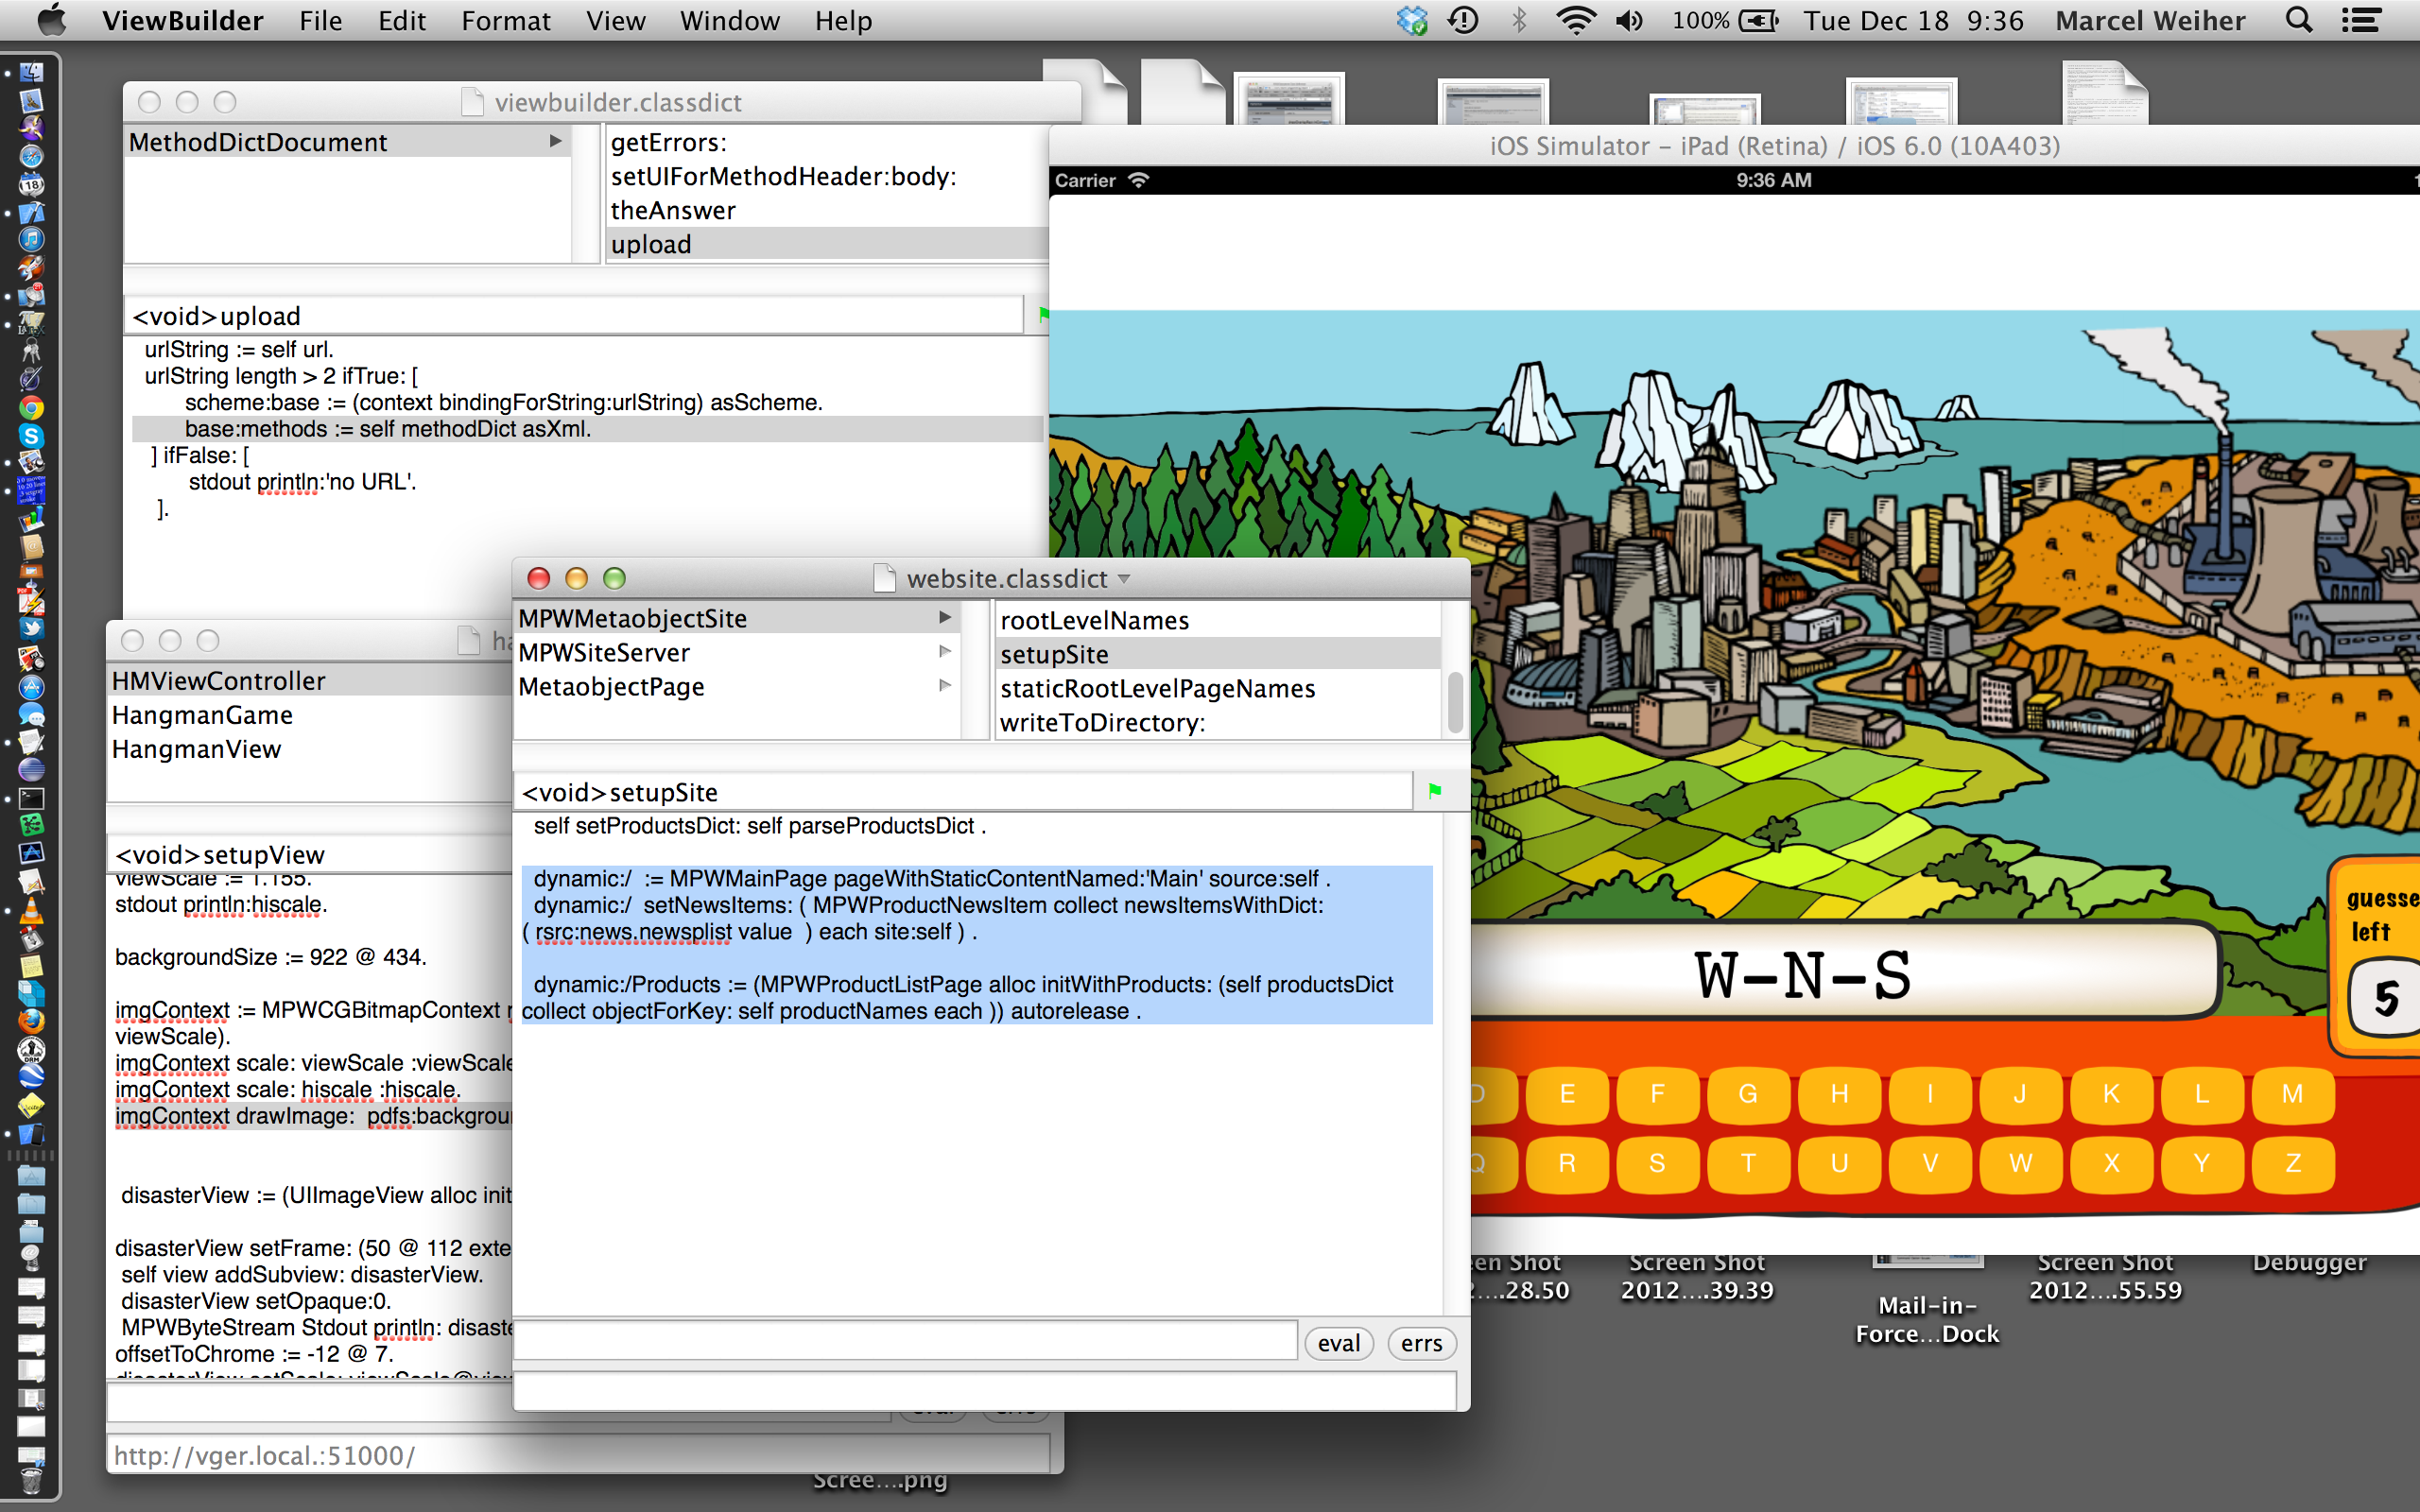
\includegraphics[scale=0.32,page=1]{PolymorphicIdentifiersInUse.png}
\caption{Polymorphic Identifiers in use}
\label{pi-inuse}
\end{figure}


The game has a large number of graphical assets that could be used much more simply in code by using special schemes for accessing app
resources, though the overall impact was not very high due to large amounts of layout logic. 
 The IDE was initially completely written in Objective-C, but dealing with remote resources was so cumbersome that
those parts were rewritten using Objective-Smalltalk with Polymorphic Identifiers.

The application that gained most from Polymorphic Identifiers was the site generator:  the asset pipeline consisting of static
content, templating mechanism, dynamic content and a page cache could be directly expressed as a series of connected
scheme-handlers.  The object that dynamically generates the site's root is placed there using the simple assignment: {\tt dynamic:/  := MPWMainPage \dots}.


\subsection{Performance}

Like plain identifiers and messages, Polymorphic Identifiers benefit from having the compiler perform
at least the character-to-reference conversion step of identifier lookup, yielding performance 
improvements over string-based identifiers.

\sloppy
Figure~\ref{var-speed} compares evaluating the identifier {\tt var:stream/target/target} with evaluating the  
equivalent string-based identifier (using Cocoa KVC): \\  { \centering {\tt [stream valueForKeyPath:@"target.target"]}. }
\fussy

We use the underlying Objective-C implementation for both the reference and its 
comparison because Objective-Smalltalk is currently an interpreted environment with
a simple AST-walker, so interpretation overhead makes performance differences in
the underlying lookup disappear.  Tests were run on a 2012 MacBook Pro 13" with 2.9 GHz Core i7 processor, the
code was self-timing using the {\tt getrusage()} call.  

%\vspace{-4.0em}
\begin{figure}
%  \centering
\begin{minipage}[c]{0.38\textwidth}
\begin{tabular}{|r|r|r|r|r|r|r|r|r|r|r|r|} \hline
Accesses  & KVC& {\tt var:}   & ratio	\\ 
 & ($\mu$s) & ($\mu$s) & \\ \hline
1 & 14 & 10 & 1.4   \\ % \hline
10 & 22 & 10 &   2.2 \\   % \hline
100 & 100 & 14 &  7.0\\   % \hline
1000 & 1227 & 29 &  42.3  \\  % \hline
10000 & 8345 & 186 &   44.9 \\   % \hline
100000 & 73036 & 1730 &    42.2 \\ \hline
\end{tabular}
\end{minipage}
\begin{minipage}[c]{0.39\textwidth}
\includegraphics[scale=0.5,page=2]{kvc-vs-var.pdf}
\end{minipage}
\vspace{-2.0em}
\caption{Time for  {\tt var:} scheme vs. \emph{Key Value Coding} for two-element path access, log scale}
\label{var-speed}
\end{figure}

For large number of operations, access via the {\tt var:} scheme (or more precisely its reference) is
around 40 times faster than using Key Value Coding, confirming our expectations about the benefits
of partial compile-time evaluation versus string-interpretation at run-time.  

In order to test the overhead of scheme-handlers, especially composite scheme-handlers, we turn
to the ability to bridge scheme-handlers to servers briefly mentioned in Section~\ref{common-reference-behavior}.
We exported three different schemes via http and then used the {\tt wrk} http-performance testing tool to stress
test the resulting http servers, using apache as a benchmark to validate our results.  Tests were run on a 2012 MacBook Pro 13" with 2.9 GHz Core i7 processor.

Figure~\ref{http-server-speed} shows the results.  Serving a specific directory using a relative scheme parametrized
with the file scheme resulted in a performance level of around 19K requests per second.  Adding the same memory cache
we used for the caching http client scheme improves performance to 23K requests per second and finally exporting a pure
memory scheme yields the best performance at 31K requests per second.   Apache has many more features and so
has slightly lower performance.

\begin{figure}
\begin{minipage}[c]{0.58\textwidth}
\begin{tabular}{|l|c|c|} \hline
Server   &  Requests/s    \\ \hline
apache & 	14876	      \\ % \hline
home-scheme (file+relative) &  19231   \\ % \hline
home-scheme (+cached)  &  23398  \\ % \hline
memory-scheme (only) &  31491  \\ \hline
\end{tabular}
\end{minipage}
\begin{minipage}[c]{0.58\textwidth}
\includegraphics[scale=0.38,page=2]{server-perf.pdf}
\end{minipage}
\vspace{-2.0em}
\caption{Performance of different schemes bridged to http vs. apache}
\label{http-server-speed}
\end{figure}



%-=-=-=-=-=-=-=-=-=-=-=-=-=-=-=-=-=-=-=-=-=-=-=-=-=-=-=-=-=-=-=-=-=-=-=%


\section{Related Work}
\label{related-work}


We already saw in Section~\ref{direct-reference} that messaging can be used for resource
access in lieu of plain identifiers.  Self~\cite{UngarS87} and Newspeak~\cite{Bracha:2010:MON:1883978.1884007} take this
approach to its logical conclusion by making all identifiers message-sends and therefore late-bound, eliminating
all nouns and replacing them with verbs\footnote{Literals are the exception}.  Although
this elimination of variables as a simplification is conceptually elegant, it leads to problems of scattering and tangling of code we
mentioned, and  ``left a complexity that bothers us to this day''~\cite{Ungar:2007:SEL:1238844.1238853}.
Handling the assignment part of resource access leads to ad-hoc rules and mechanisms to tie together
the slot accessor methods that Ungar and Smith say ``troubled us a bit''~\cite{Ungar:2007:SEL:1238844.1238853}.

Polymorphic Identifiers are a result of the same basic premise that identifiers should always be late-bound.  However,
it doesn't follow the apparent implicit assumption that only messaging can be late-bound and therefore identifiers must
be messages in order to be late-bound, and the related assumption that interfaces must be message-based.

This assumption certainly doesn't apply to the World Wide Web and the REST architectural style~\cite{fielding-rest}, where
it is (universal) resource identifiers that are the interfaces, and messaging is the hidden implementation detail.  This 
approach is taken to its logical extreme by  by Resource Oriented Computing~\cite{roc},
which encodes all computation into identifiers, with an {\tt action:} scheme that is ``a functional programming language encoded as a URI''.

Although scheme-handlers can be exported via http, Polymorphic Identifiers leave the decision of whether to present a messaging
or a resource-based interface to the developers,
similar to properties in C\#~\cite{Archer:2001:IC:516715} and Objective-C 2.0~\cite{Kochan:2009:PO:1538451}, which closely match the proposal in~\cite{Spinellis:2002:MPC:510857.510868}.  Properties are syntactic sugar for a pair of accessor methods and allow clients to use 
 plain identifiers syntax to access values via message-sends, including assignment for setting the value.   However, properties
 are just syntactic sugar for one type of resource access, they are not user-extensible like Polymorphic Identifiers 
 and don't integrate access to external resources or first class references.

Common LISP~\cite{Steele:1990:CLL:95411} has {\tt symbol-macrolet}, which was explicitly limited to lexical scoping due to fears 
that having simple identifiers with overloaded meaning could be confusing~\cite{gabriel-lisp-identifiers}, echoing similar concerns by the creators
of Smalltalk-72 of syntax that was too flexible~\cite{Kay:1996:EHS:234286.1057828}.  Having clear syntactic markers in the form of scheme-prefixes
and directly associating each prefix with one scheme-handler in Polymorphic Identifiers avoids confusion as to the meaning of specific identifiers.

The E language~\cite{MillerRobustComposition}  supports URI-Expressions as a direct language feature using angle brackets for access to 
resources such as files using and to the underlying Java classes:   {\tt $\langle$file:/home/marcs/myFile.txt$\rangle$},  \\ {\tt $\langle$unsafe:java.util.makeCalendar>.getYEAR()$\rangle$}.

E even allows custom schemes to be defined, but  only for read-access, separate from other identifiers and without the ability to extract references.

A different approach to resource access comes from the operating system community:  Plan9 
integrates a wide variety of local and remote~\cite{plan9network} resources and services into a single directory tree~\cite{plan9names} that is made available on a per-process basis, but mediated by the kernel and accessed only indirectly via system calls and string-based
identifiers.
User level filesystems like FUSE~\cite{fuse} or the BSD Pass-to-User-Space~\cite{kantee:puffs} 
system bring some of these ideas to commercial operating systems, but make these filesystems visible globally to all
processes on a machines. 


Polymorphic Identifiers are similar to Embedded Domain Specific Languages~\cite{edsl}
in that they allow domain-specific language elements to be added to a language, rather
than having to create a completely new language with an external DSL or attempt to 
achieve the desired effect with an internal DSL\cite{fowlerdsl}.  

Like polymorphic embedding of DSLs~\cite{polydsl}, Polymorphic Identifiers allow
a single syntax to be used with multiple, pluggable semantic interpretations permitting
composition of functionality~\cite{embeddeddsl}.  However, Polymorphic Identifiers
are applicable to general purpose programming languages, not just DSLs, while
at the same time restricting their focus to the identifiers used.




%-=-=-=-=-=-=-=-=-=-=-=-=-=-=-=-=-=-=-=-=-=-=-=-=-=-=-=-=-=-=-=-=-=-=-=%

\section{Summary and Outlook}
\label{summary-and-outlook}

We have created Polymorphic Identifiers, a generalization of identifiers based on URI
syntax and extensible, pluggable semantics based on scheme-handlers.   
Polymorphic Identifiers allow any type of resource that can be addressed via URI
to be directly referenced, avoiding the need to create and use string-based identifiers 
to access these resources, and providing compiler support for these identifiers.

The uniformity of the syntax and the use of common interfaces for scheme-handlers
enables polymorphic behavior for resource access, permitting different scheme-handlers
to be substituted without affecting client code. Application-specific schemes
enable abstraction.
Custom scheme-handlers can be implemented as normal objects and added
to the language, or even composed from pre-existing handlers and
combinators.

With the user-extensible identifier architecture of Polymorphic Identifiers, it becomes possible to add abstraction
and information-hiding capabilities to identifiers and expand the use of REST-style
programming beyond network and Web-environments.



%\section*{Acknowledgements}

%The authors would like to thank Carl Friedrich Bolz, Gilad Bracha, Richard Gabriel, and Michael Perscheid for their
%helpful feedback.

%-=-=-=-=-=-=-=-=-=-=-=-=-=-=-=-=-=-=-=-=-=-=-=-=-=-=-=-=-=-=-=-=-=-=-=%

%\appendix
%\section{Appendix A}

%This is the text of the appendix, if you need one.

%\acks

%Acknowledgments, if needed.

% We recommend abbrvnat bibliography style.

\vfill
\break

\bibliographystyle{abbrvnat}
\bibliography{polymorphic-identifiers}


% The bibliography should be embedded for final submission.

\balancecolumns

\end{document}
